\documentclass{article}
\usepackage[utf8]{inputenc}
\usepackage[margin=1in]{geometry}
\usepackage{amsmath, amsfonts}
\usepackage{fancyhdr}
\usepackage{multicol}
\usepackage{graphicx}
\usepackage[inline]{enumitem}
\usepackage{wrapfig}
\graphicspath{ {images/} }
\pagestyle{empty}
\fancyhf{}
\cfoot{\thepage}
\pagenumbering{gobble}

\lhead{MATB42: Assignment \#8}
\rhead{
Poon, Keegan\\
1002423727\\
Mar 20th 2018}
\newcommand{\norm}[1]{\| #1 \|}
\newcommand{\deriv}[1]{\frac{d}{d #1}}
\newcommand{\parti}[1]{\frac{\partial}{\partial #1}}
\renewcommand{\headrulewidth}{0pt}
\newcommand{\gam}{\boldsymbol{\gamma}}
\begin{document}

\thispagestyle{fancy}
\begin{enumerate}
    \begin{multicols}{2}
    \item A surface $S$ is obtained by rotation the given figure in the $xy$-plane about the $z$-axis. (The arc is part of a circle of radius 1 centered at (2,0).)
        \begin{enumerate}
            \item Paratemetrize $S$ (in pieces) and compute the surface area.

            We have that the upper line when rotated, can be parametrized by a restricted cone and similarly for the bottom. The top and bottom respectively can be written as 
        \end{enumerate}
            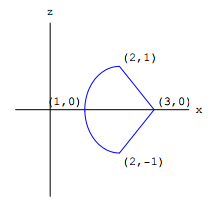
\includegraphics[width=0.25\textwidth]{b42-a8-q1ex}
    \end{multicols}
    \[ \boldsymbol \Phi (u,\theta) = ((1-u)3 \cos \theta, (1-u)3 \sin \theta, 3u) ,\; 0\leq u \leq 1,\, 0 \leq \theta \leq 2\pi\] 
    \[ \boldsymbol \Phi (u,\theta) = ((1+u)3 \cos \theta, (1+u)3 \sin \theta, -3u) ,\; -1 \leq u \leq 0 ,\, 0 \leq \theta \leq 2\pi\] 

    For the circular portion to the left, when rotated around, it will be the inner half of a torus, so the equation will be

    (b) Use a computer algebra system to sketch $S$.
    \newpage

    \item Let $S$ be the cone with vertex (2,3,3) and base the circle $x^2 + y^2 = 1$ in the $xy$-plane.
        \begin{enumerate}
            \item Paratemetrize $S$
            Starting with a base of a circle, we get $(\cos \theta, \sin \theta, 1)$ with $0 \leq \theta \leq 2\pi$. To change into a cone multiply $x$ and $y$ by $(1-u)$ with $0 \leq u \leq 1$ and finally to shift the vertex, add $(2u, 3u, 2u)$ where $z = 2u$ since the base equation already has a 1, so $1 + ku <= 3 \implies k \leq 2$.
            \[ \implies \boldsymbol \Phi (u,\theta) = ( (1-u)\cos \theta + 2 u, (1-u)\sin \theta + 3u, 1 + 2u) \] 
            \item Use a computer algebra system to sketch $S$.
            \item Write down the integral that would give the surface area of $S$. (You are not expected to evaluate the integral.)
            \begin{align*}
                \boldsymbol \phi_\theta &= (-(1-u)\sin \theta,\, (1-u)\cos \theta,\,0) \\
                \boldsymbol \phi_u &= (-\cos \theta + 2,\, -\sin\theta + 3,\,2) \\
                \boldsymbol \phi_\theta \times \boldsymbol \phi_u &= ((2(1-u)\cos \theta),  (2(1-u)\sin \theta),  \\ 
                & \; (-(1-u)\sin \theta)(-\sin \theta + 3) - ((1-u)\cos\theta)(-\cos \theta + 2)) \\
                &= ((2-2u)\cos \theta,  (2-2u)\sin \theta, (1-u)\sin^2 \theta -(3 - 3u)\sin \theta + (1-u)\cos ^2 \theta - (2-2u)\cos \theta) \\
                &= ((2-2u)\cos \theta,  (2-2u)\sin \theta, (1-u)-(3 - 3u)\sin \theta - (2-2u)\cos \theta) \\
                \norm{ \boldsymbol \phi_\theta \times \boldsymbol \phi_u} &= \sqrt{(2-2u)^2\cos^2 \theta +  (2-2u)^2\sin^2 \theta + ((1-u)-(3 - 3u)\sin \theta - (2-2u)\cos \theta)^2} \\
                &= \sqrt{(2-2u)+ ((1-u)-(3 - 3u)\sin \theta - (2-2u)\cos \theta)^2} \\
                \implies \mathcal{A}(S) &= \int_0^1\int_0^{2\pi} \sqrt{(2-2u)+ ((1-u)-(3 - 3u)\sin \theta - (2-2u)\cos \theta)^2}\, d\theta \, du \\
            \end{align*}
        \end{enumerate} 

    \newpage

    \item Let $S$ be the self-intersecting rectangle in $\mathbb{R}^3$ given by the implicit equation $x^2-y^2z=0.$
        \begin{enumerate}
            \item Give a parametrization of $S$ and use a computer algebra system to provide a sketch.

            \[x^2 - y^2z = 0 \implies y^2z = x^2 \implies z = \bigg(\frac{x}{y}\bigg)^2\]
            \[\boldsymbol \Phi (x,y) = (x, y, \bigg(\frac{x}{y}\bigg)^2\]
            \item Is your parametrization one-to-one? Explain.
            \item Find the equation of the tangent plane to $S$ at $\displaystyle \bigg( \frac{1}{4}, \frac{1}{2}, \frac{1}{4} \bigg).$
        \end{enumerate}  
    \item Let $S$ be the surface defined by $x^2 + y^2 = 1$ for $0 \leq z \leq 1$ and by $x^2 + y^2 = z^2$ for $1 \leq z \leq 2$.
        \begin{enumerate}
            \item Use symbolic algebra software to sketch $S$.
            \item Evaluate $\displaystyle \int_S \boldsymbol F \cdot \, d \boldsymbol S $ where $\boldsymbol F (x,y,z) = (-y,x,z)$ and $S$ is oriented by outward pointing normals.
        \end{enumerate}  
        \begin{enumerate}
            \item Evaluate the (vector) surface integral $\displaystyle \int_S \boldsymbol F \cdot \, d \boldsymbol S$ in each of the following cases.
                \begin{enumerate}
                    \item $\boldsymbol F (x,y,z) = (1,x,z),\; S$ is the upper hemisphere $x^2+y^2+z^2 = 1,\, z \geq 0,$ with $\boldsymbol n $ pointing upward.
                    \item $\boldsymbol F (x,y,z) = (2,x,z+y) ,\; S$ is that part of the plane $x+y+z = 1$ which lies in the first octant and $\boldsymbol n$ points upward.
                    \item Marsden \& Tromba, page 425, \#22.
                \end{enumerate}
        \end{enumerate}
        
    \item Let $S$ be the portion of the plane $x-2y+z=1$ that is cut off by the coordinate planes and the plane $x+y=1$. Let $\boldsymbol V$ be the velocity field $\boldsymbol V (x,y,z) = (y,z,x^2)$. Find the flow across $S$ when $\boldsymbol n$ points upward. Explain your answer.

    \item Let $S$ be the closed surface that consists of the hemisphere $x^2+y^2+z^2 = 1,\, z \geq 0,$ and its base $x^2 + y^2 \leq 1,\, z = 0.$ let $\boldsymbol E$ be the electric field $\boldsymbol E(x,y,z) = (2x,2y,2z).$ Directly calculate the electric flux across $S$.
        
\end{enumerate}
\end{document}

